\documentclass[12pt]{article}
\usepackage[right=1in,left=1in,top=1in,bottom=1in]{geometry}
\PassOptionsToPackage{hyphens}{url}
\usepackage{hyperref}
\hypersetup{colorlinks, citecolor=blue, filecolor=blue, linkcolor=blue, urlcolor=blue}
\usepackage{graphicx}
\usepackage{url}
\usepackage[round, authoryear, comma, sort]{natbib}
\bibliographystyle{aer}
\usepackage{amsmath, amsthm, bbm} 
% \usepackage[fleqn]{amsmath}
\usepackage{engord}
\usepackage{float}
\usepackage{subfig}
\usepackage{pdflscape}
\usepackage{multirow}
\usepackage{booktabs}
\usepackage{dcolumn}
\usepackage{siunitx}
\usepackage{pgfplots}
\usepackage{minted}
\pgfplotsset{compat=1.14}
\pgfplotsset{every axis label/.append style={font=\tiny}}
\usepackage[labelsep=period, labelfont=bf]{caption} %% This switches "Table 1: Title" to "Table 1. Title"
\captionsetup{font=footnotesize}
\usepackage{tabularx}
% \usepackage{subcaption}
% \renewcommand{\thesection}{\Roman{section}} 
% \renewcommand{\thesubsection}{\thesection.\Roman{subsection}}

\usepackage{floatrow}

% \usepackage{lmodern}
% \usepackage[defaultsans]{cantarell}
% \renewcommand{\familydefault}{\sfdefault}
% \renewcommand{\sfdefault}{lmss}
% \usepackage[T1]{fontenc}
% \renewcommand*\familydefault{\sfdefault}
\usepackage[T1]{fontenc}
\renewcommand*\familydefault{\sfdefault} 
% \usepackage{sansmathfonts}
% 
% Font
% \usepackage[T1]{fontenc}
% \usepackage{lmodern}
% \usepackage{dsfont,mathrsfs,ushort}
\usepackage{mathpazo}

\usepackage{amssymb} %% Necessary, just for the \checkmark command  in tables.
\usepackage{multirow} %% Necessary if we are doing tables in LaTeX

\usepackage{xr}

\usepackage{adjustbox}

\usepackage{setspace}
\setstretch{1.2}
% \onehalfspacing
% \linespread{1.5}

\usepackage{sectsty}
\sectionfont{\large}
\subsectionfont{\normalsize}
\subsubsectionfont{\normalsize}

\newcommand\ddfrac[2]{{\displaystyle\frac{\displaystyle #1}{\displaystyle #2}}}
\newcommand{\specialcell}[2][c]{\begin{tabular}[#1]{@{}l@{}}#2\end{tabular}}
\newtheorem{theorem}{Theorem}
\newtheorem{definition}{Definition}


%% Tables
\makeatletter
\newcommand{\armultirow}[3]{%
  \multicolumn{#1}{#2}{%
    \begin{picture}(0,0)%
      \put(0,0){%
        \begin{tabular}[t]{@{}#2@{}}%
          #3%
        \end{tabular}%
      }%
    \end{picture}%
  }%
}%

\newcolumntype{f}{>{$}l<{$}}
\newcolumntype{n}{l}
\newcolumntype{N}{>{\scriptsize}l}
\newcolumntype{v}[1]{>{\raggedright\hspace{0pt}}p{#1}}
\newcolumntype{V}[1]{>{\scriptsize\raggedright\hspace{0pt}}p{#1}}
%
% array.sty, dcolumn.sty
\newcolumntype{B}[1]{>{\boldmath\DC@{.}{,}{#1}}l<{\DC@end}}
\newcolumntype{d}[1]{>{\DC@{.}{,}{#1}}l<{\DC@end}}
\newcolumntype{i}[1]{>{\DC@{.}{,}{#1}\mathnormal\bgroup}l<{\egroup\DC@end}}
\newcolumntype{s}[1]{>{\DC@{.}{,}{#1}\mathsf\bgroup}l<{\egroup\DC@end}}
%
% array.sty, rotating.sty
\newcolumntype{R}[1]{%
  >{\begin{turn}{90}\begin{minipage}{#1}\scriptsize\raggedright\hspace{0pt}}l%
  <{\end{minipage}\end{turn}}%
}
%
% array.sty, tabularx.sty
\newcolumntype{x}{>{\scriptsize\raggedright\hspace{0pt}}X}
\makeatother

%%%%%%%%%%%%%%%%%%%%%%%%%%%%%%%%%%%%%%%%%%%%%%%%%%%%%%%%%%%%%

\title{ \vspace*{-2.5cm} \hspace*{-0.5cm} The Missing Reallocation Effect: \\ Decomposing The Declining Labour Share\footnote{
I am deeply indebted to my supervisors Agnieszka Markiewicz and Eric Bartelsman for their guidance and continued support. I thank Georg Duernecker, Miguel Le\'on-Ledesma, Benjamin Moll, \'Akos Valentinyi, and Erasmus School of Economics seminar participants for their excellent comments and suggestions. 
}}

\author{Elliott Weder\thanks{Erasmus University Rotterdam and Tinbergen Institute. My email:
\href{mailto:weder@ese.eur.nl}{weder@ese.eur.nl}}}

\date{ \vspace*{0.5cm} December, 2023\\
% \textbf{Preliminary and Incomplete. \\ Please do not circulate.}
} 

%%%%%%%%%%%%%%%%%%%%%%%%%%%%%%%%%%%%%%%%%%%%%%%%%%%%%%%%%%%%%

\begin{document}

\bgroup
\let\footnoterule\relax

\begin{singlespace}
\maketitle
\end{singlespace}

\begin{abstract}
    \noindent Since the mid-1980s, the US labour share fell considerably and the economy reallocated towards sectors with high labour shares. Previous studies claim this reallocation does not play a role in the decline of the labour share, so aggregate movements should be understood primarily as a within-sector phenomenon. By exploiting a decomposition method that explicitly accounts for simultaneous changes in the relative size of sectors and sectoral labour shares, I show reallocation offsets around half of the aggregate labour share decline - an order of magnitude larger than previous studies. My results imply that sectoral labour shares cannot be studied in isolation to gain insights into the fall of the aggregate labour share, the cause of which is not yet agreed upon in the literature. 
    % WRITE MORE ABOUT UNDER- AND OVER-COUNTING??
\end{abstract}


\thispagestyle{empty}

\clearpage
\egroup
\setcounter{page}{1}



%%%%%%%%%%%%%%%%%%%%%%%%%%%%%%%%%%%%%%%%%%%%%%%%%%%%%%%%%%%%%%%%%
\section{Introduction\label{sec:introduction}}
Since the mid-1980s, the US labour share fell considerably. Figure \ref{fig:labour_shares} shows a clear downward trend for four measures of the labour share after 1987 \footnote{Section \ref{sec:data} discusses the four methods I use to measure the labour share.}. A large macroeconomic literature has attempted to uncover the mechanisms driving the shift in the distribution of income away from labour, yet no clear consensus has been reached.


\begin{figure}[h]
    \centering
    \caption{\normalsize Aggregate labour share decline relative to 1987, percentage point change}
    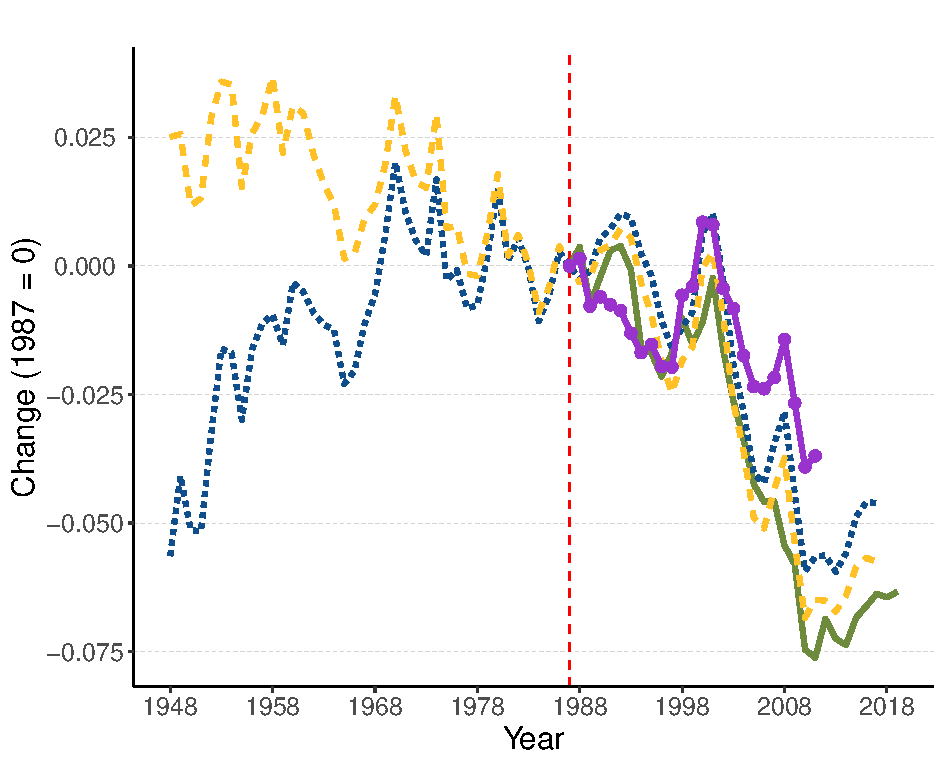
\includegraphics[width=10cm]{Introduction/diff_labour_shares.pdf}

    \label{fig:labour_shares}

\begin{minipage}{\linewidth}
    \caption*{\textit{Notes}: The aggregate labour share equals labour income (self-employed labour income + payroll labour income) divided by GDP. The labour income of self-employed individuals is imputed four different ways. Section \ref{sec:data} contains the data description. \\
    \textit{Source}: Bureau of Economic Analysis (BEA), Bureau of Labour Statistics (BLS), and author's calculations.}
\end{minipage}
\end{figure}

\noindent The decline in the labour share coincided with a substantial reallocation of value-added towards sectors with high labour share levels, mainly in services \citep{boppartStructuralChangeKaldor2014, herrendorfTwoPerspectivesPreferences2013, gagglStructuralChangeProduction2023, bridgmanLaborShareMarkups2023}. All else equal, such reallocation should counterfactually raise the labour share, as the aggregate reflects the higher labour shares in the growing sectors to a greater extent. How much of the declining labour share is due to reallocation between sectors with different labour share levels and how much arises due to labour shares changing within sectors? 

Despite the reallocation towards industries with high labour shares, numerous studies, including \citet{daoWhyLabourReceiving2019a, elsbyDeclineLaborShare2013a} and \citet{karabarbounisGlobalDeclineLabor2014a}, argue that between-sector compositional changes do not play a role in the decline of the US labour share, so aggregate movements should be understood primarily as a within-sector phenomenon. In this paper, I show that the apparent lack of a reallocation effect is due to the specific decomposition method used in previous studies. First, I theoretically compare the commonly used shift-share (between-within) decomposition to the \citet{haltiwangerMeasuringAnalyzingAggregate1997} (between-within-cross) decomposition (henceforth, I refer to it as the `Haltiwanger decomposition'). The two methods are closely related because they both decompose the same change in the aggregate labour share. However, the additional cross term in the Haltiwanger decomposition explicitly captures the impact of covarying sectoral weights (relative size) and sectoral labour shares on the aggregate labour share. I theoretically show the shift-share between- and within-sector contributions include half of the Haltiwanger cross term. Therefore, the shift-share decomposition unintentionally counts half of the covariance impact as between-sector reallocation. The same holds for the within-sector contribution. 

% Specifically in the US context, 

% Adjusting for the effect of the covariance is important in the US context in which the reallocation towards high labour share sectors interacts with sector-specific levels and trends in labour shares.  

% The reallocation effect is missing in previous studies by virtue of the decomposition method used. 

Second, I show the cross contribution is large and negative using US industry data and four different measures of the labour share. Following my theoretical result, the between- and within-sector contributions measured using the shift-share decomposition are downward biased because half of the negative covariance is added to each. Decomposing the declining payroll labour share using the shift-share method attributes only 4\% to reallocation and the remaining 96\% to within-sector mechanisms. A shift-share decomposition implies that to explain the path of the aggregate labour share one needs only to examine the determinants of labour shares within sectors. However, using the Haltiwanger decomposition - which removes the impact of co-movement between sectoral weights and sectoral labour shares - reallocation accounts for -47\% of the total decline. The Haltiwanger decomposition recovers the positive reallocation effect missing from previous studies. In addition, the impact of within-sector mechanisms falls from 96\% to 45\% when using the Haltiwanger decomposition. I find similar results for three other measures of the aggregate labour share. The Haltiwanger decomposition highlights the quantitative importance of three channels operating in tandem to depress the labour share: reallocation towards industries with high labour share levels, declining labour shares within sectors, and the negative co-movement between sectoral weights and sectoral labour shares. 

% need 'missing reallocaion effect' here
% need to talk about the size of the cross term
% need to talk about the three channels emerging 

 
 % THE NEW THING IS THAT CROSS TERMS ARE ALSO IMPORTANT ---> EXPLAINING 100\% OF THE DECLINE WHILE THE OTHER TWO CANCEL OUT... ALSO MENTION THE SELF-EMPLOYED 

\vspace{0.3cm}

\textbf{Related Literature.} The negligible reallocation effect found in previous studies leads to authors proposing within-sector mechanisms to explain the falling labour share. Falling sectoral labour shares are related to the increased adoption of automation \citep{acemogluAutomationNewTasks2019}, rising concentration \citep{barkaiDecliningLaborCapital2020}, intermediate inputs prices \citep{castro-vincenziIntermediateInputPrices2022}, and sectoral heterogeneity in trade exposure \citep{elsbyDeclineLaborShare2013a}. Why these mechanisms would not also cause reallocation between sectors is not clear. For instance, increased trade exposure with China displaced manufacturing employment and automation is likely to promote growth heterogeneously across sectors that benefit differently from its adoption \citep{autorChinaSyndromeLocal2013, acemogluAutomationNewTasks2019}. Since I find that reallocation and co-movements between sectors' size and labour shares are also important channels affecting the aggregate labour share, a methodology flexible enough to accommodate both is necessary to parse out which of the above mechanisms is driving the decline in the labour share. 

% that to parse out which factors are quantitatively important, a methodology flexible enough to incorporate the effect of each on reallocation between sectors, and, hence, co-movements between sectors' size and labour shares, is necessary. 


% While not ruling any of the literature's proposed mechanisms out, my findings suggest a unified framework incorporating reallocation and, hence, co-movements between sectors' size and labour shares can more richly explain the underlying dynamics of the aggregate labour share.

% need to talk about using frameworks that examine the same factors but allow for the reallocation effect to be measured... 

\citet{bridgmanLaborShareMarkups2023} and \citet{feijomoreiraDeclineLaborShare2022} find a positive reallocation effect on the aggregate labour share in two-sector structural models. However, neither paper explains why their results differ from previous seminal studies claiming reallocation has no effect. My paper bridges this gap.

Lastly, \citet{autorFallLaborShare2020} and \citet{kehrigMicroLevelAnatomyLabor2021a} decompose changes in sectoral labour shares at the establishment level using US Census data. The authors explicitly measure the impact of co-movement between establishments' size (reallocation) and their labour shares on different industries' labour shares. Both papers find that co-movements drive sectoral trends. The establishment-level data allows for a more granular analysis than the industry-level data I use. However, the establishment-level data is not consistently measured across sectors, whereas the industry-level data covers the entire economy. 

% Because robust firm-level measures of value added are not avail- able from the Economic Census outside of manufacturing, we use the cruder measure of the ratio of payroll to sales. 

% it does not afford a comprehensive view of 

% the data does not cover the entire economy, coverage is not consistent and comprehensive 

% leads to a more granular analysis, but is not comprehensively cover the entire economy (consistently) 

% the authors are not able to examine the labour share of the entire economy 

% means the authors cannot examine the labour share of the entire economy. In contrast, the detailed industry-level data I use covers the entire economy. 


% The difference is made up by the large and negative cross term, which accounts for 103\% of the aggregate decline. 

% * and mention replication of previous Elsby study

% use between-within (shift-share) decompositions and claim between-sector reallocation does not offset the fall in the labour share. As a result, the authors of these papers only examine within-sector mechanisms as potential drivers of the labour share, for example by regressing sectoral trade exposure and the adoption of automation on changes in sectoral labour shares. First, it is unclear why these mechanisms would not also cause reallocation between sectors. For instance, increased trade exposure displaces manufacturing employment and automation is likely to promote growth heterogeneously across sectors that benefit differently from its adoption \citep{autorChinaSyndromeLocal2013, acemogluAutomationNewTasks2019}. Second, given the clear reallocation we see towards high labour share sectors, why is the reallocation effect missing from the results in the literature? 

% To bridge the gap, I exploit the between-within-cross decomposition from \citet{haltiwangerMeasuringAnalyzingAggregate1997}, rather than the between-within decomposition used in all previous studies in the literature. The additional cross term in the Haltiwanger decomposition explicitly accounts for co-movements in between-sector and within-sector mechanisms, which is important in the US context where reallocation coincides with sector-specific trends affecting the labour share within sectors. In the between-within decomposition, the effect coming from co-movement is split evenly across the between-sector and within-sector terms. As a result, the between-sector term, which is meant to capture the impact of reallocation, is also capturing the impact of co-movements. Using the between-within-cross decomposition, reallocation accounts for -47\% of the decline in the aggregate payroll labour share (the percentage is negative because reallocation offsets the decline). Using the between-within decomposition, reallocation accounts for 4\% of the decline, an order of magnitude smaller. The reason the results change so dramatically is the additional cross term in the Haltiwanger decomposition is large and negative and cancels out the positive between-sector effect in the between-within decomposition. Furthermore, reallocation accounts for a similar portion of the decline when accounting for self-employed individuals' labour income as well. 

% My results imply the missing reallocation effect is an artefact of the decomposition method used in previous studies. Therefore, to understand the falling labour share an integrated approach combining between-sector reallocation, within-sector mechanisms, and co-movements of the two is needed. Previous models attempting to explain the decline often ignore the notion of a sector's size and, therefore, cannot account for the reallocation channel. While not the goal of this paper, my results provide realistic calibration targets for models of the declining labour share incorporating all three channels. Furthermore, \citet{grossmanElusiveExplanationDeclining2022} argue the falling labour share has been explained ``many times over'' by the literature, due to the focus only on factors leading to its decline. My results help to partly reconcile their point because reallocation partially offsets the decline. 

 % \citet{elsbyDeclineLaborShare2013a, barkaiDecliningLaborCapital2020, daoWhyLabourReceiving2019a, castro-vincenziIntermediateInputPrices2022, acemogluAutomationNewTasks2019} and \citet{karabarbounisGlobalDeclineLabor2014a} all propose various within-sector mechanisms to explain the fall in the labour share. Examples include regressing sectoral trade exposure, adoption of automation, rising concentration, and rising intermediate input prices on labour shares within sectors. The reason they examine mechanisms at the sectoral level is standard shift-share decompositions measure the effect of reallocation to be negligible. First, the proposed mechanisms are also likely to lead to reallocation between sectors, as mentioned before. Second, my results indicate reallocation is also a relevant channel for the aggregate labour share, and, therefore, should also be incorporated. In this way, my paper complements the pre-existing literature. 



\section{Data\label{sec:data}}
The aggregate labour share in year $t$, $\lambda_{t}$, can be written as the weighted sum of $N$ sectoral labour shares
\begin{equation}
    \lambda_{t} = \sum_{i=1}^{N}\omega_{it}\lambda_{it}.
\label{eqn:weighted_ls}
\end{equation}
The sectoral weights and labour shares are defined as
\begin{equation}
    \omega_{it} = \frac{VA_{it}}{\sum_{i=1}^{N}VA_{it}}
\end{equation}
and 
\begin{equation}
   \lambda_{it} = \frac{WL_{it}}{VA_{it}} 
\end{equation}
in which $VA_{it}$ and $WL_{it}$ denote sector $i$'s gross value-added and labour income, respectively, in year $t$. I use value-added data from the Bureau of Economic Analysis (BEA) industry accounts. Labour income in sector $i$ in year $t$ equals the sum of payroll workers' labour income $WL_{it}^{p}$ and self-employed persons' labour incomes $WL_{it}^{s}$. The first is measured using payroll tax records. However, the labour-capital split is not recorded for self-employed persons' total income. How should labour income be divided from returns on capital investments for self-employed individuals? Following the literature, I exploit four different assumptions for imputing self-employed labour income, resulting in the four labour share definitions I use throughout the paper. 

The first is the `same-wage-distribution' approach used in the BEA-BLS integrated industry-level production account \citep{eldridgeBEABLSIntegratedIndustrylevel2020}. First, assume the average wages for self-employed individuals and payroll workers are equal within skill$\times$demographic cells $j$, for each sector $i$ and year $t$. Second, the labour income $WL_{jit}^{s}$ of self-employed individuals equals the labour income of payroll workers $WL_{jit}^{p}$ corrected by the ratio of hours worked (which are recorded for both)
\begin{equation}
    WL_{jit}^{s} = WL_{jit}^{p} \times \frac{L_{jit}^{s}}{L_{jit}^{p}}
\end{equation}
in which $L_{jit}^{p}$ and $L_{jit}^{p}$ correspond to the total hours worked for payroll workers and self-employed individuals in cell $j$, sector $i$ and year $t$, respectively. Second, the `same-labour-share' approach by \citet{mendieta-munozDeclineUSLabor2021} corrects total self-employed individuals' income $Y_{it}^{s} \equiv WL_{it}^{s} + RK_{it}^{s}$ (the labour-capital split is not known) by the payroll labour share $\frac{WL_{it}^{p}}{VA_{it}}$
\begin{equation}
    WL_{it}^{s} = \frac{WL_{it}^{p}}{VA_{it}} \times Y_{it}^{s}.
\label{eqn:same_labour_share}
\end{equation}
Third, the `economy-wide labour share' assumption subtracts the total self-employed persons' income from the denominator in the payroll labour share in equation (\ref{eqn:same_labour_share})
\begin{equation}
    WL_{it}^{s} = \frac{WL_{it}^{p}}{VA_{it} - Y_{it}^{s}} \times Y_{it}^{s}.
\label{eqn:economy_wide}
\end{equation}
Lastly, since the first three definitions impute self-employed persons' labour income, they are subject to potential measurement error. To avoid mismeasurement, I examine the payroll labour share $\frac{WL_{it}^{p}}{VA_{it}}$. The payroll labour share represents the part of the aggregate labour share which is unambiguously labour income. 

The final choice required to specify $\omega_{it}$ and $\lambda_{it}$ is the level at which sectors $i$ are defined. Aggregating the economy into fewer sectors reduces the extent to which reallocation can affect the aggregate labour share. For example, reallocation across NAICS 3-digit industries is always measured as a within-sector contribution if the industries are within the same NAICS 2-digit classification, even if the labour shares are constant within the 3-digit industries\footnote{Appendix \ref{fig:minormajor} demonstrates that aggregating NAICS 3-digit sectors into NAICS 2-digit classifications eliminates the entire between-sector effect, even though the effect is positive at the 2-digit level.}. Therefore, aggregating the economy into coarser sectors loads onto the within-sector contribution. Ideally, I would use establishment-level information, but this kind of data is generally not available for the universe of firms in the US economy, and only within certain major sectors. To compromise, and for comparison to previous studies, I use sectors classified at the NAICS 3-digit classification for the `same-wage-distribution' and `payroll labour share' measures. For the `same-labour-share' and `economy-wide' assumptions, I can only use data aggregated into 14 sectors because total self-employed income $Y_{it}^{s}$ is not measured at a more disaggregated level. Table \ref{tab:data} shows how the average sectoral labour share falls from the first 5 years to the last 5 years for each of the four labour share definitions. 


\begingroup
\renewcommand*{\arraystretch}{1.3}

\begin{table}[h]
    \centering
    \small
    \caption{\normalsize Average sectoral labour share for each definition.}
    \begin{tabular}{l|cccc}
        
        \toprule[1.1pt]
        
        Measure & Mean (first five) & Mean (last five) & Years & Number of sectors \\

        \midrule[1.1pt]

        Same-wage-distribution & 0.69 & 0.61 & 1987-2019 & 60 \\

        Same-labour-share & 0.69 & 0.65 & 1987-2017 & 14 \\

        Economy-wide & 0.78 & 0.68 & 1987-2017 & 14 \\

        Payroll & 0.65 & 0.62 & 1987-2011 & 60 \\

        \bottomrule[1.1pt]
    \end{tabular}

\begin{minipage}{\linewidth}
\captionsetup{justification=raggedright,singlelinecheck=false}
    \caption*{Source: see Appendix \ref{sec: data source} for the data sources of each measure.}
\end{minipage}
    \label{tab:data}
\end{table}

\endgroup


\section{The Missing Reallocation Effect\label{sec:puzzle}}
I now use the industry-level data to demonstrate why the absence of a reallocation effect in previous studies is puzzling. The aggregate labour share in year $t$, $\lambda_{t}$, can be written as the weighted sum of sectoral labour shares
\begin{equation}
\begin{split}
    \lambda_{t} &= \sum_{i=1}^{N}\omega_{it}\lambda_{it}
\end{split}
\label{eqn:weighted_ls_second}
\end{equation}
in which $\omega_{it}$ denote a sector's value-added-to-GDP weight in year $t$, and $\lambda_{it}$ is sector $i$'s labour share of value-added.

\noindent First, towards which sectors does the economy reallocate since 1987? The left panel in figure \ref{fig:GS} shows the share of value-added shifted towards service-producing industries since 1987, which is already well documented in the literature (e.g. \citet{herrendorfTwoPerspectivesPreferences2013, bridgmanLaborShareMarkups2023}). Second, how do labour share levels and trends differ between growing and shrinking sectors? The right panel shows the average labour share in services sectors is higher and declines slower than in goods sectors. Goods-producing industries see a much sharper drop in their average labour share from 1987 onwards. All else equal, the reallocation of value-added towards higher labour share sectors in services should partially offset the decline in the labour share. Indeed, in the right panel of figure \ref{fig:GS}, the fall in the aggregate labour share is muted relative to the larger decline in the average labour share in goods-producing sectors.


\begin{figure}[h]
  \centering
    \caption{\normalsize Value-added and average labour shares of goods and services.}
  \subfloat{\label{fig:b}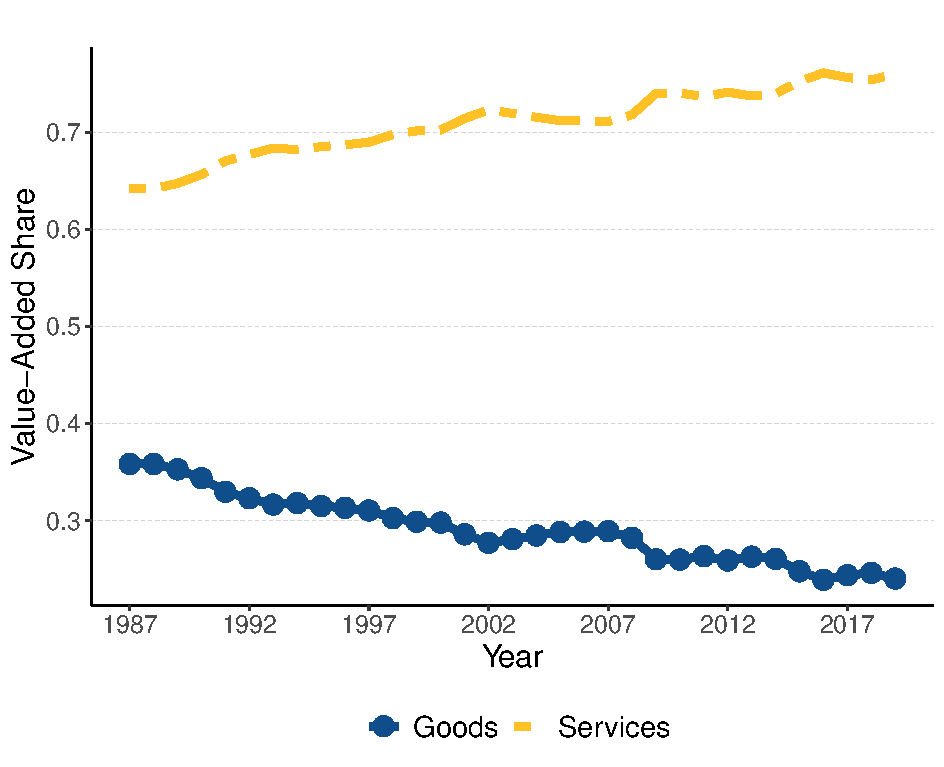
\includegraphics[width=.45\linewidth]{Puzzle/omega_GS.pdf}}
  \subfloat{\label{fig:c}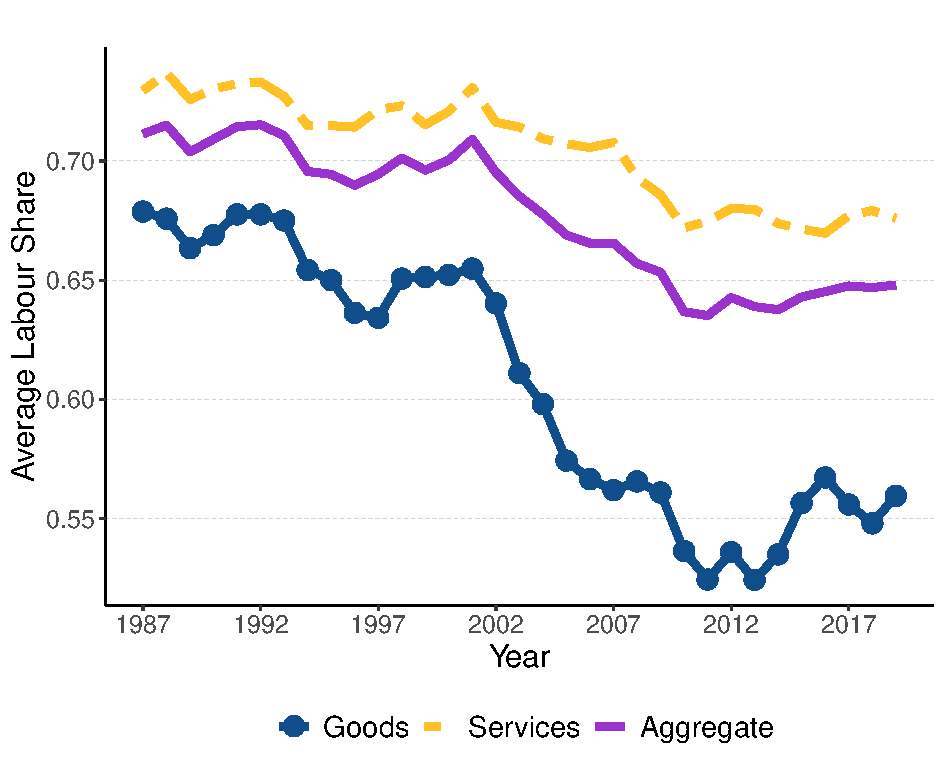
\includegraphics[width=.45\linewidth]{Puzzle/lambda_GS.pdf}}\vfill

    \label{fig:GS}

\begin{minipage}{\linewidth}
    \caption*{\textit{Notes}: The left panel shows the value-added-to-GDP share of goods and service sectors. The right panel shows the average labour share within goods and service sectors. \\
    \textit{Source}: BEA-BLS integrated industry-level production account and author's calculations.}
\end{minipage}
\end{figure}


Third, I conduct a simple counterfactual exercise in which I fix sectoral labour shares $\lambda_{it}$ at their 1987 values, allowing only the weights $\omega_{it}$ to change. The counterfactual labour share is given by
\begin{equation}
    \lambda_{t}^{\text{counterfactual}} = \sum_{i=1}^{N}\omega_{it}\lambda_{i1987}.
\label{eqn:counterfactual_ls}
\end{equation}
Figure \ref{fig:counterfactual_index} shows the counterfactual path of each labour share definition, all indexed to the 1987 aggregate labour share. For all four definitions, albeit to different extents, the counterfactual labour share is higher than the actual path. These counterfactuals suggest the labour share would have risen since 1987 if only sectoral weights (reallocation) had changed since then. Why is the positive reallocation effect missing from decompositions used in previous studies? To answer the question, in the next section I describe the the decomposition framework I apply to the industry data. 


\begin{figure}[h]
    \centering
    \caption{\normalsize Counterfactual labour shares holding sectoral labour shares fixed}
    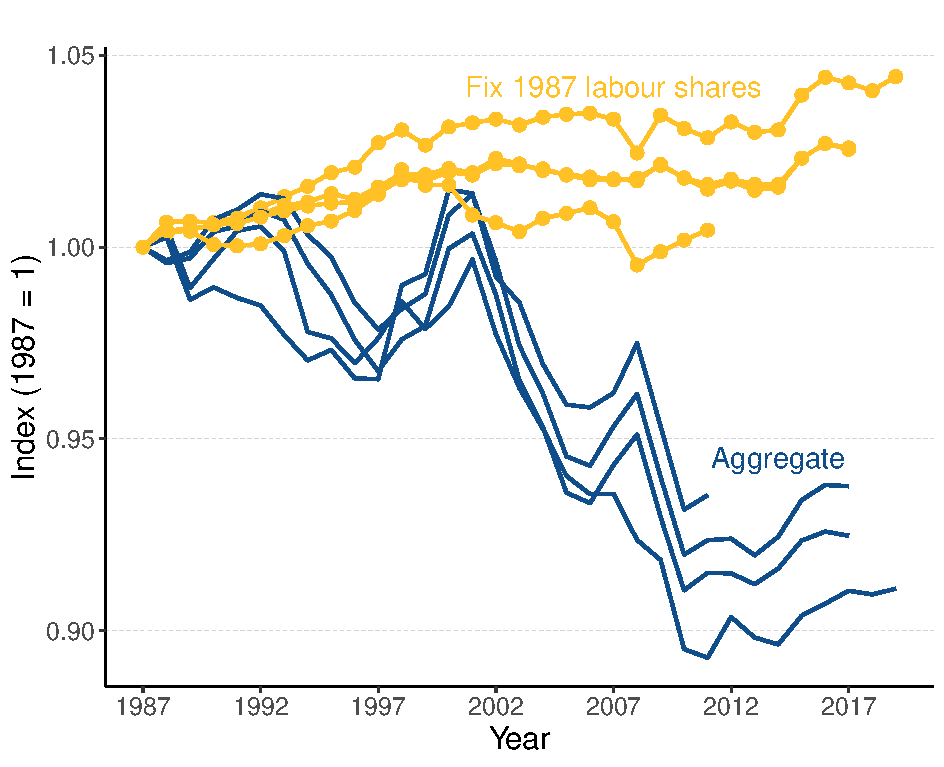
\includegraphics[width=10cm]{Puzzle/counterfactual_graph_index.pdf}

    \label{fig:counterfactual_index}

\begin{minipage}{\linewidth}
    \caption*{\textit{Notes}: The four lines sloping downward represent the path of the aggregate labour share for the four methods I use to impute self-employed labour income. The four lines sloping upward show the counterfactual paths of the aggregate labour share had sectoral labour shares stayed fixed at their 1987 values: $\lambda_{t}^{\text{counterfactual}} = \sum_{i=1}^{N}\omega_{it}\lambda_{i,1987}$. All lines are indexed to the respective 1987 labour share. \\
    \textit{Source}: Bureau of Economic Analysis (BEA), Bureau of Labour Statistics (BLS), and author's calculations.}
\end{minipage}
\end{figure}






\section{Decomposition Framework\label{sec:framework}}
How much of the declining labour share arises due to reallocation between sectors with different labour share levels and how much comes from labour shares changing within sectors? I use both the shift-share and the Haltiwanger decomposition to decompose changes in the aggregate labour share. Most studies of the declining labour share use the shift-share method, whereas the Haltiwanger decomposition has not been used to the best of my knowledge.  

Using the weighted-average definition of the labour share in equation (\ref{eqn:weighted_ls_second}), the shift-share method decomposes changes in the labour share, $\Delta \lambda_{t} = \lambda_{t} - \lambda_{t-1}$, into a term capturing reallocation, arising from $\Delta\omega_{it}$, and a term capturing the effect of changing sectoral labour shares, derived from $\Delta\lambda_{it}$.
\begin{definition}[Shift-Share Decomposition]
    The change in the labour share, $\Delta \lambda_{t} = \lambda_{t} - \lambda_{t-1}$, can be decomposed into two terms
    \begin{equation}
        \Delta \lambda_{t} = \underbrace{\sum_{i=1}^{N}\Delta\omega_{it}\tilde{\lambda}_{it}}_\text{Between} + \underbrace{\sum_{i=1}^{N}\tilde{\omega}_{it}\Delta\lambda_{it}}_\text{Within} 
    \label{eqn:shift_share_decomposition}
    \end{equation}    
    in which $\Delta x_{it} = x_{it} - x_{it-1}$ and $\tilde{x}_{it} = \ddfrac{x_{it-1} + x_{it}}{2}$.
\end{definition}
\noindent Both terms in the shift-share decomposition keep the bases defined at their arithmetic means $\tilde{\lambda}_{it}$ and $\tilde{\omega}_{it}$, respectively. Alternatively, the Haltiwanger decomposition uses bases defined at their $t-1$ values and, therefore, splits changes in the aggregate labour share into a between, within, and cross term. 

\begin{definition}[Haltiwanger Decomposition]
    The change in the labour share, $\Delta \lambda_{t} = \lambda_{t} - \lambda_{t-1}$, can be decomposed into three terms
    \begin{equation}
        \Delta \lambda_{t} = \underbrace{\sum_{i=1}^{N}\Delta\omega_{it}\lambda_{it-1}}_\text{Between} + \underbrace{\sum_{i=1}^{N}\omega_{it-1}\Delta\lambda_{it}}_\text{Within} + \underbrace{\sum_{i=1}^{N}\Delta\omega_{it}\Delta\lambda_{it}}_\text{Cross}
    \label{eqn:haltiwanger_decomposition}
    \end{equation}
    in which $\Delta x_{it} = x_{it} - x_{it-1}$.
\end{definition}
\noindent Using either decomposition, the `Between' term is used to measure the effect of reallocation between sectors with different labour shares. The `Within' terms capture the effect of changing labour shares within industries. The `Cross' term in the Haltiwanger decomposition captures the impact of co-movement of sectoral weights and labour shares. Theorem \ref{theorem_1} demonstrates how the two decompositions are related since they are both exact decompositions of changes in the labour share $\Delta\lambda_{t}$. 

\begin{theorem}
\label{theorem_1}
By adding half of the Haltiwanger cross term to the Haltiwanger between-sector term, you get the shift-share between term.
\begin{equation*}
    \underbrace{\sum_{i=1}^{N}\Delta \omega_{it} \tilde{\lambda}_{it}}_\text{Shift-Share Between} = \underbrace{\sum_{i=1}^{N}\Delta  \omega_{it} \lambda_{it-1}}_\text{Haltiwanger Between} + \frac{1}{2}\underbrace{\sum_{i=1}^{N}\Delta \omega_{it} \Delta \lambda_{it}}_\text{Haltiwanger Cross}.
\end{equation*}
The same relationship holds for the within-sector terms.
\begin{equation*}
    \underbrace{\sum_{i=1}^{N}\tilde{\omega}_{it}\Delta \lambda_{it}}_\text{Shift-Share Within} = \underbrace{\sum_{i=1}^{N}\omega_{it-1}\Delta \lambda_{it}}_\text{Haltiwanger Within} + \frac{1}{2}\underbrace{\sum_{i=1}^{N}\Delta \omega_{it} \Delta \lambda_{it}}_\text{Haltiwanger Cross}.     
\end{equation*}
\end{theorem}
\begin{proof}
    See Appendix \ref{sec: theorem_1_proof}.
\end{proof}
\noindent Theorem \ref{theorem_1} demonstrates the shift-share between-sector term, which aims to capture the effect of reallocation, also captures half of the impact of co-movements between $\omega_{it}$ and $\lambda_{it}$. The same logic applies to the within-sector terms. Moreover, a non-zero Haltiwanger cross term leads to different conclusions about the impact of between-sector reallocation and within-sector mechanisms depending on the decomposition method used. For example, suppose the Haltiwanger between-sector term is positive, which means reallocation leads to a counterfactually higher aggregate labour share. Using the shift-share decomposition instead can result in a zero reallocation effect being measured if the Haltiwanger cross term is large and negative, because it subtracts from the positive Haltiwanger between-sector term, via Theorem \ref{theorem_1}. Additionally, the negative cross term leads to negative within-sector mechanisms being overcounted. Therefore, the Haltiwanger decomposition provides a more suitable measure of reallocation and within-sector causes when sectoral weights and labour shares covary, as I will show in the next section using the industry-level data.

% Empirically, the cross term is large and negative, as I show in the next section. Using the shift-share decomposition measures a zero reallocation effect, but the Haltiwanger decomposition recovers a positive effect. Moreover, the shift-share decomposition overcounts the negative within-sector contribution. 

Furthermore, the Haltiwanger method is preferable to the shift-share method when there are trends in either $\lambda_{it}$ or $\omega_{it}$. For instance, a downward trend in $\lambda_{it}$ pushes the arithmetic mean, $\tilde{\lambda}_{it}$, down each period, meaning the shift-share between term captures reallocation and sector-level trends in labour shares (a within-sector phenomenon). \citet{diez-catalanLaborShareService2018, elsbyDeclineLaborShare2013a} and \citet{gutierrezInvestigatingGlobalLabor2017} show the labour share is trending down in virtually every sector and rising in a few. The presence of sectoral trends does not pose an issue when using the Haltiwanger decomposition because the bases are fixed at the previous period values. 

By examining only the shift-share and Haltiwanger decompositions, I omit several other commonly used decomposition techniques. For example, changes in the aggregate labour share can also be decomposed as in  \citet{olleyDynamicsProductivityTelecommunications1996}. I use the shift-share method since it is typically used in studies that decompose the declining labour share. Moreover, I use the Haltiwanger method because, as Theorem \ref{theorem_1} shows, it is closely related to the shift-share method, but additionally accounts for co-movements between sectors' weights and labour shares.  






\section{Decomposition Results\label{sec:empirics}}
Here I decompose the four series of the aggregate labour share using both the shift-share and Haltiwanger methods for the industry-level data. 


% In figures \ref{fig:decomp_1}, \ref{fig:decomp_2to3} and \ref{fig:decomp_4}, I plot the cumulative path of the Between, Within, and Cross terms estimated for each year. 

\subsection{Payroll Labour Share}
I begin by decomposing the payroll labour share. The advantage of examining the payroll labour share is that payroll labour income represents the part of the labour share accruing unambiguously to labour. Figure \ref{fig:decomp_1} shows the cumulative paths of the between, within, and cross terms estimated for each year using both the shift-share and Haltiwanger decomposition. 

The left panel in figure \ref{fig:decomp_1} shows the cumulative between-sector terms for each decomposition. The shift-share decomposition replicates the results from \citet{elsbyDeclineLaborShare2013a} and estimates that between-sector reallocation adds a cumulative -0.1pp to the labour share from 1987 to 2011, around 4\% of the total decline. Using the shift-share decomposition, one would conclude there is a zero reallocation effect. However, the cross effect estimated in the Haltiwanger decomposition is negative and growing over time. Via Theorem \ref{theorem_1}, a negative cross term reduces the shift-share between-sector term relative to the Haltiwanger between-sector term. The Haltiwanger decomposition estimates that reallocation cumulatively adds 1.7pp to the payroll labour share, around -47\% of the total decline. The Haltiwanger decomposition recovers a positive reallocation effect, in line with the counterfactual evidence presented in Section \ref{sec:puzzle} and in contrast to previous studies. 

Moreover, the negative within-sector contribution in the shift-share decomposition is overestimated due to the negative cross term. In the right panel, The shift-share decomposition apportions 96\% of the total decline in the labour share to within-sector mechanisms, whereas the Haltiwanger decomposition apportions only 45\%. Since the between, within, and cross contributions add up to 100\%, the Haltiwanger decomposition implies co-movements between sectoral weights and labour shares account for 102\% of the decline in the labour share. The negative co-movement between $\omega_{it}$ and $\lambda_{it}$ is the dominant factor in the declining payroll labour share. 

% * and then do the variance decomposition with respect to wl and va (have to use price indexes??)


\begin{figure}[h]
  \centering
\caption{\normalsize Cumulative decomposition of the payroll labour share}
\subfloat[Between-sector contributions]{\label{fig:elsby_hw}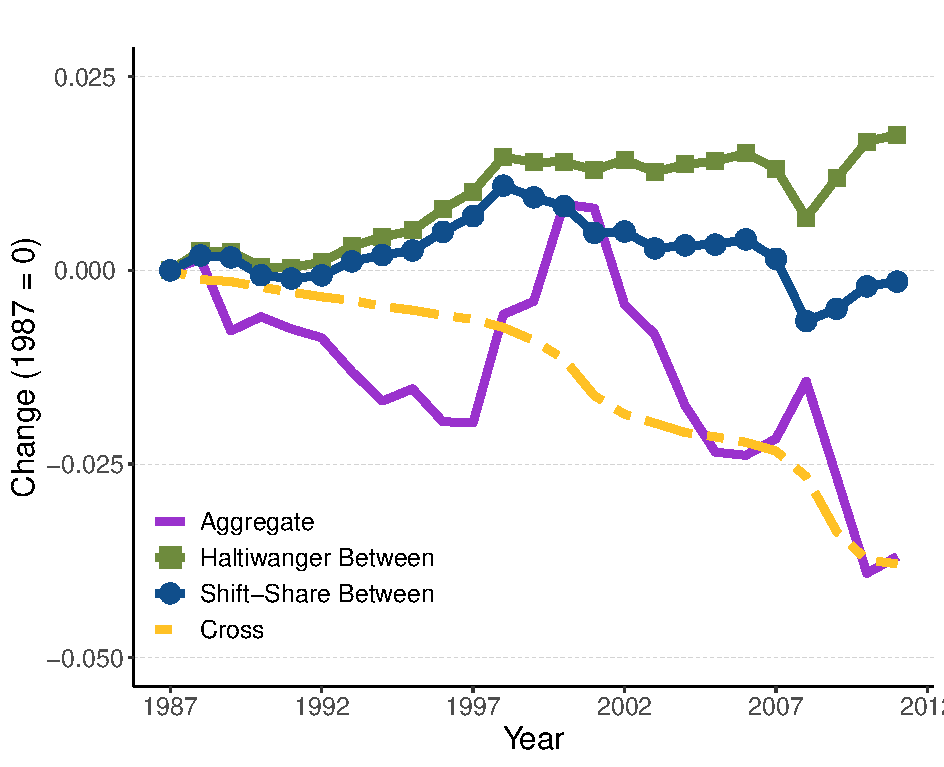
\includegraphics[width=.45\linewidth]{Decomposition/elsby_Between_D_graph.pdf}}
\subfloat[Within-sector contributions]{\label{fig:elsby_hw}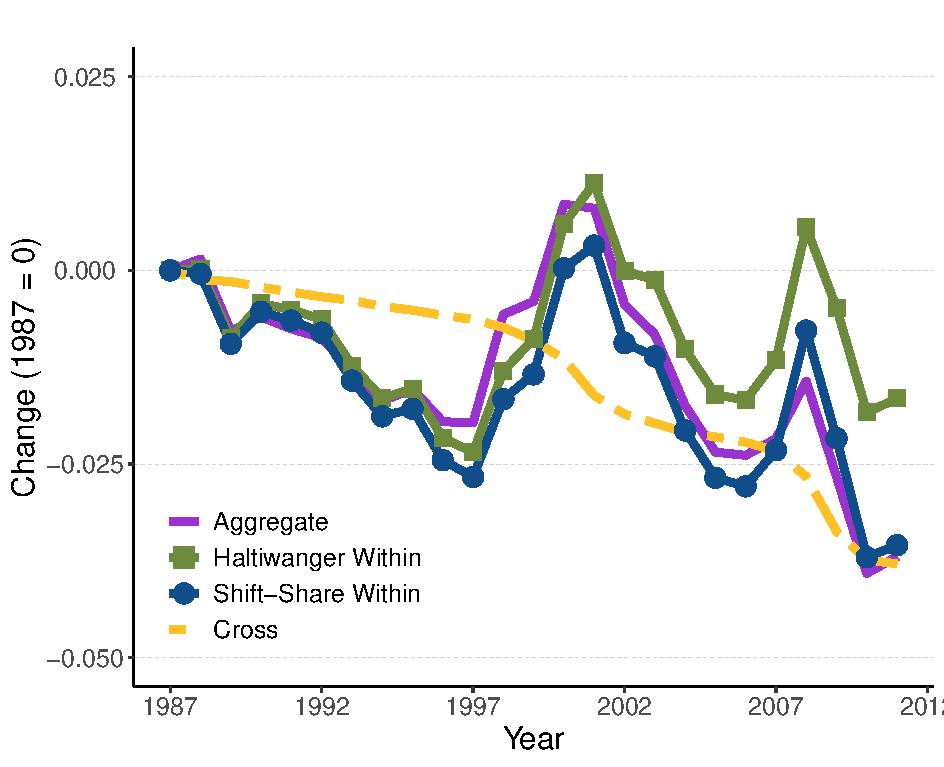
\includegraphics[width=.45\linewidth]{Decomposition/elsby_Within_D_graph.pdf}}\vfill
\begin{minipage}{\linewidth}
    \caption*{\textit{Notes}: Cumulative between, within and cross terms for both decomposition methods using the `payroll labour share' approach, 1987 to 2011. `0.05' on the y-axis corresponds to 5 percentage points (pp). The Aggregate and Cross lines are equivalent across both panels. \\
    \textit{Source}: BEA, \citet{elsbyDeclineLaborShare2013a} replication package, and author's calculations.}
\end{minipage}
\label{fig:decomp_1}
\end{figure}

The Haltiwanger cross term is negative since changes in value-added affect sectoral weights and sectoral labour shares in opposite directions: $VA_{it}$ appears in the numerator and denominator, respectively. Appendix \ref{sec: veil} shows the cross term is negative for virtually every sector analysed. 
% Furthermore, Appendix \ref{} demonstrates the variance in sectoral labour shares in each year is largely accounted for by the covariance between sectoral labour income $WL_{it}$ and sectoral value-added $VA_{it}$, rather than the variance of $WL_{it}$ or $VA_{it}$ by itself. 
Given the quantitative importance of the cross term, my results imply value-added dynamics within sectors are important for the path of the aggregate payroll labour share. \citet{kehrigMicroLevelAnatomyLabor2021a} report a similar finding using establishment-level data in the US manufacturing sector. 


\subsection{Accounting For Self-Employed Labour Income}

While the payroll labour share captures the part of the aggregate labour share accruing unambiguously to labour income, how do the results differ when self-employed labour income is accounted for? Figures \ref{fig:decomp_2}, \ref{fig:decomp_3}, and \ref{fig:decomp_4} plot the cumulative shift-share and Haltiwanger decompositions for the three self-employed labour income imputation methods I use. In contrast to the `payroll labour share' results, all three shift-share decompositions estimate a positive and non-negligible reallocation effect. Looking at the three left panels in figures \ref{fig:decomp_2}, \ref{fig:decomp_3}, and \ref{fig:decomp_4}, between-sector changes add to the aggregate labour share measures. Nevertheless, each panel shows the cross effect is negative, so, as a result, the shift-share decomposition undercounts the positive reallocation effect and overcounts the negative within-sector effect. Netting out the impact of the co-movement, the Haltiwanger decomposition lines show that reallocation adds between 14.5pp and 27.7pp more to the aggregate labour share than the shift-share method estimates. Similarly, the Haltiwanger decomposition estimates that declining labour shares within sectors account for between 14.5pp and 27.7pp less than the shift-share method estimates. 

Table \ref{tab:rr} indicates the number of percentage points that the shift-share decomposition undercounts the effect of reallocation and overcounts the effect of declining labour shares within sectors relative to the Haltiwanger decomposition. Regardless of the labour share definition, using the shift-share method severely undercounts the positive effect of reallocation and loads onto the within-sector contribution. From the cumulative Haltiwanger decompositions in figures \ref{fig:decomp_1}, \ref{fig:decomp_2}, \ref{fig:decomp_3}, and \ref{fig:decomp_4}, the quantitative importance of all three channels - between, within, and cross - for changes in the aggregate labour share emerges. Sectoral labour shares cannot be studied in isolation to examine the decline of the aggregate labour share. 

% The large and negative cross term for each labour share variation leads to a positive between-sector term being undercounted and a negative within-sector term being overcounted when using the shift-share decomposition. In Table \ref{tab:rr} I indicate by how many percentage points the under- and overcounting occurs. Depending on the definition of the labour share used, the shift-share decomposition undercounts a positive between-sector term by between 14.5 and 51.3 percentage points. Since Theorem \ref{theorem_1} shows the cross term is split evenly across the shift-share between- and within-sector terms, the negative within-sector contribution is overcounted by between 14.5 and 51.3 percentage points. Regardless of the labour share definition used, there is considerable under- and overcouting occurring. 



{\setstretch{1.0}

\begin{figure}[h]
  \centering
\caption{\normalsize Cumulative decompositions of aggregate labour share}
\subfloat[Between-sector]{\label{fig:klems_hw}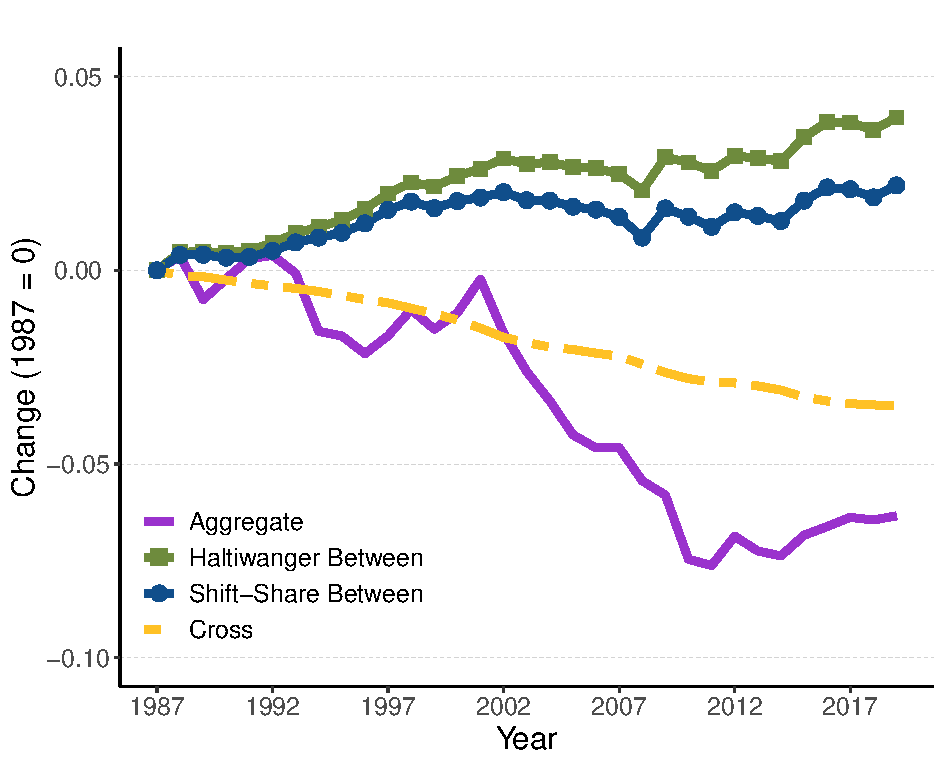
\includegraphics[width=.45\linewidth]{Decomposition/Between_D_graph.pdf}}
\subfloat[Within-sector]{\label{fig:klems_hw}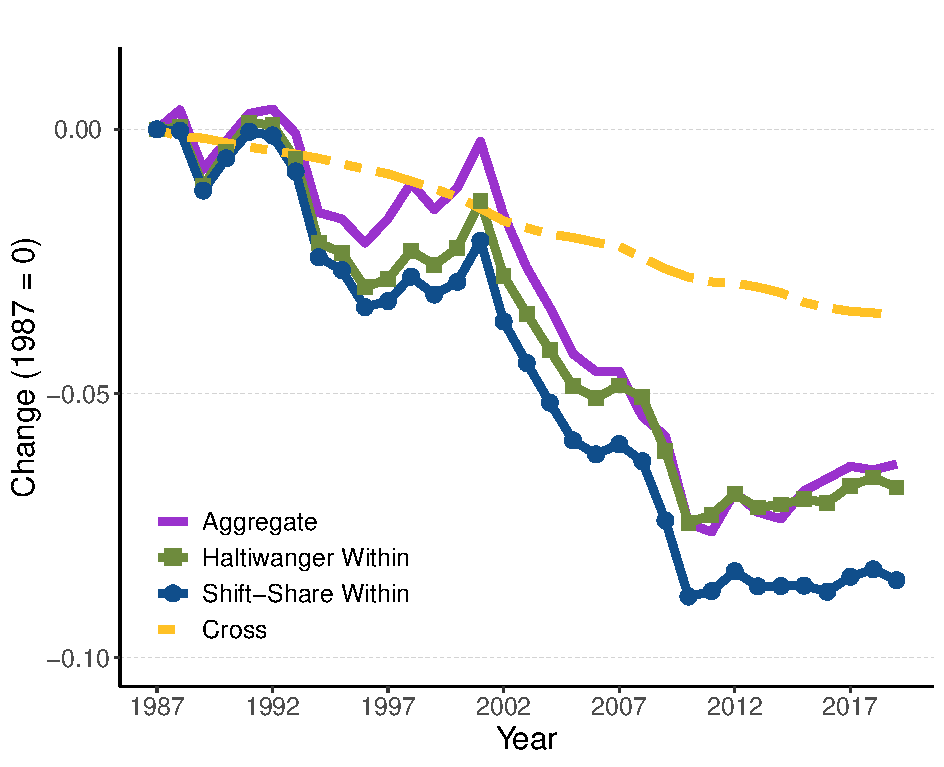
\includegraphics[width=.45\linewidth]{Decomposition/Within_D_graph.pdf}}\vfill
\begin{minipage}{\linewidth}
    \caption*{\textit{Notes}: Cumulative between, within and cross terms for both decomposition methods using the `same-wage-distribution' assumption, 1987-2019. `0.05' on the y-axis corresponds to 5 percentage points (pp). The scale of the left and right panels are different, but the Aggregate and Cross lines are equivalent. \\
    \textit{Source}: BEA-BLS integrated industry-level production account and author's calculations.}
\end{minipage}
\label{fig:decomp_2}
\end{figure}
}

\begin{figure}[h]
  \centering
\caption{\normalsize Cumulative decompositions of aggregate labour share}
\subfloat[Between-sector]{\label{fig:mm_ss}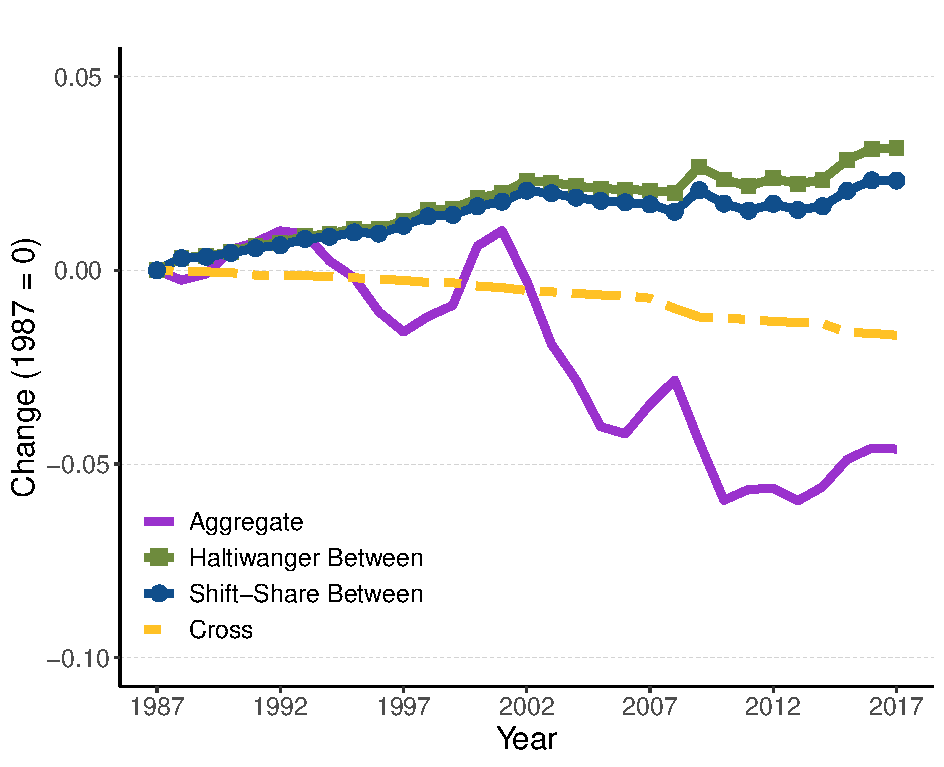
\includegraphics[width=.45\linewidth]{Decomposition/mm_Between_D_graph.pdf}}
\subfloat[Within-sector]{\label{fig:mm_hw}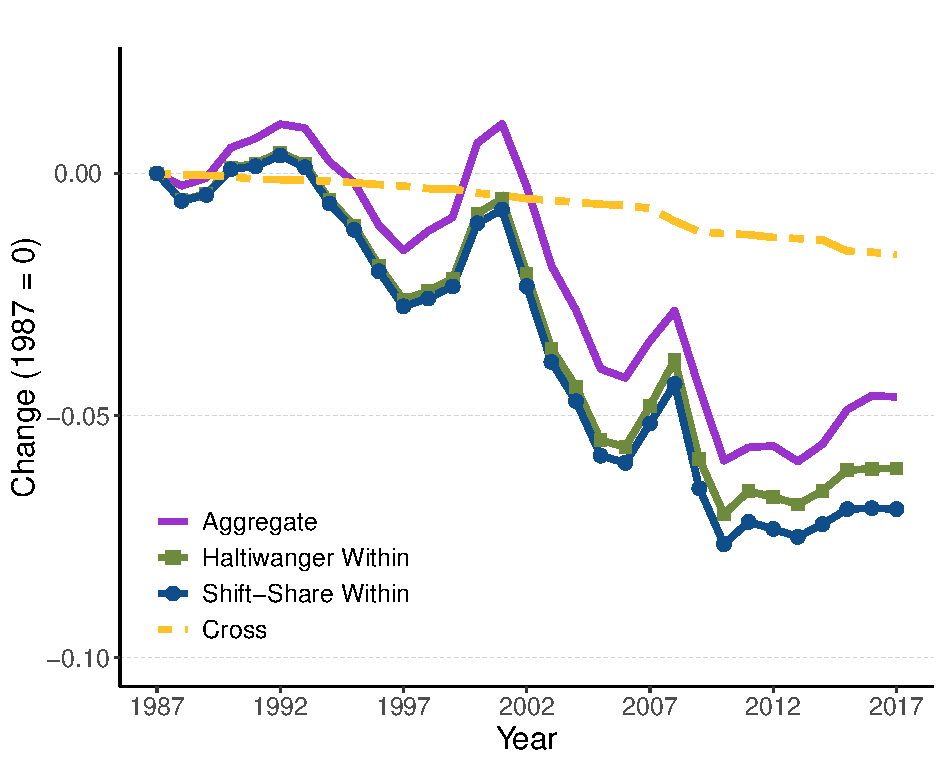
\includegraphics[width=.45\linewidth]{Decomposition/mm_Within_D_graph.pdf}}\vfill
\begin{minipage}{\linewidth}
    \caption*{\textit{Notes}: Cumulative between, within and cross terms for both decomposition methods using the `same-labour-share' assumption, 1987-2017. `0.05' on the y-axis corresponds to 5 percentage points (pp). The scale of the left and right panels are different, but the Aggregate and Cross lines are equivalent. \\
    \textit{Source}: BEA, BLS, \citet{mendieta-munozDeclineUSLabor2021} replication package, and author's calculations.}
\end{minipage}
\label{fig:decomp_3}
\end{figure}

\begin{figure}[h]
  \centering
\caption{\normalsize Cumulative decompositions of aggregate labour share}
\subfloat[Between-sector]{\label{fig:ew_ss}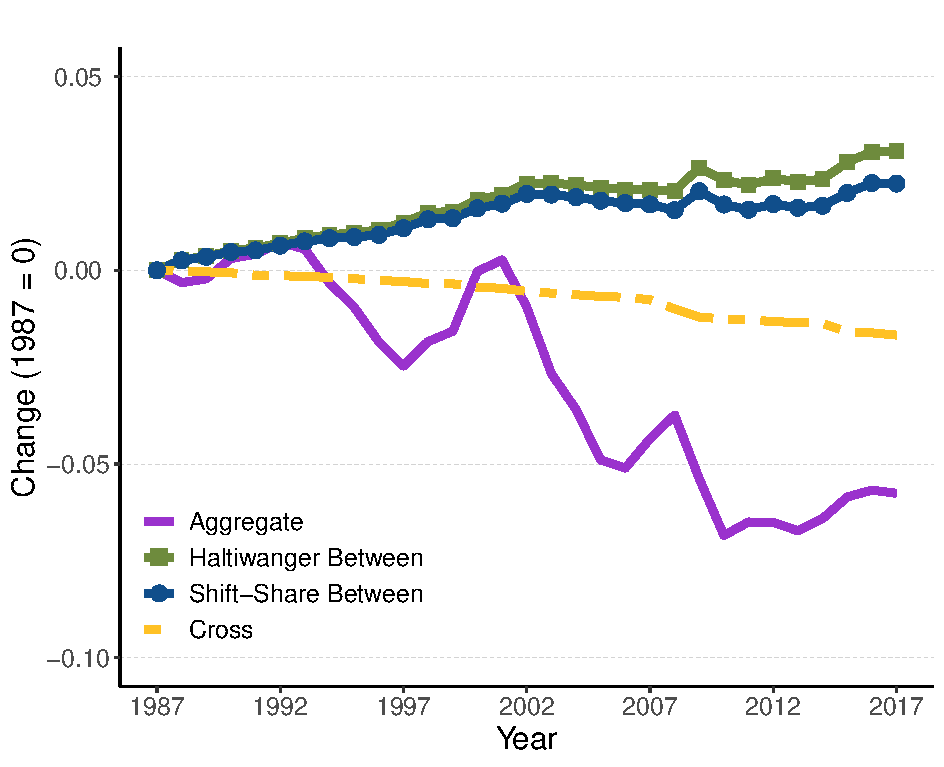
\includegraphics[width=.45\linewidth]{Decomposition/ew_Between_D_graph.pdf}}
\subfloat[Within-sector]{\label{fig:ew_hw}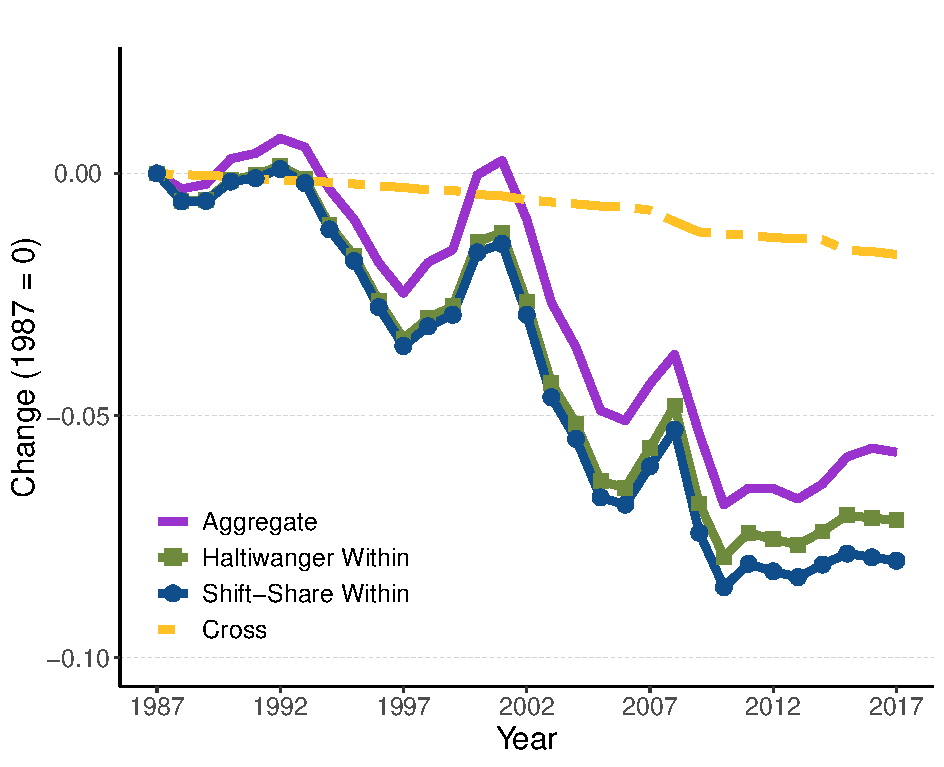
\includegraphics[width=.45\linewidth]{Decomposition/ew_Within_D_graph.pdf}}\vfill
\begin{minipage}{\linewidth}
    \caption*{\textit{Notes}: Cumulative between, within and cross terms for both decomposition methods using the `economy-wide labour share' assumption, 1987-2017. `0.05' on the y-axis corresponds to 5 percentage points (pp). The scale of the left and right panels are different, but the Aggregate and Cross lines are equivalent. \\
    \textit{Source}: BEA, BLS, \citet{mendieta-munozDeclineUSLabor2021} replication package, and author's calculations.}
\end{minipage}
\label{fig:decomp_4}
\end{figure}


\begin{table}[h]
    \centering
    \small
    \caption{\normalsize Percentage point under- or over-counting of shift-share relative to Haltiwanger decomposition}
    \begin{tabular}{lcc}
       \toprule[1.1pt]
        
        & Between-sector undercounted & Within-sector overcounted \\
        
        \cmidrule[0.8pt](lr{0.125em}){2-3}

       \textbf{A. Payroll labour share.} & \multirow{2}{*}{-51.3} & \multirow{2}{*}{51.3} \\
       \textit{Years}: 1987-2011 &  &  \\

       \textbf{B. Same-wage-distribution.} & \multirow{2}{*}{-27.7} & \multirow{2}{*}{27.7}\\
       \textit{Years}: 1987-2019 &  &  \\

       \textbf{C. Same-labour-share.} & \multirow{2}{*}{-18.2} & \multirow{2}{*}{18.2}\\
       \textit{Years}: 1987-2017 &  &  \\

       \textbf{D. Economy-wide.} & \multirow{2}{*}{-14.5} & \multirow{2}{*}{14.5}  \\
       \textit{Years}: 1987-2017 &  &  \\       
       \bottomrule[1.1pt]
    \end{tabular}
    
\begin{minipage}{\linewidth}
\captionsetup{justification=raggedright,singlelinecheck=false}
    \caption*{\textit{Notes}: The `Between-sector undercounted' column subtracts the percentage of the labour share decline accounted for by the shift-share between-sector term from the percentage accounted for by the Haltiwanger between term. The `Within-sector overcounted' column subtracts the shift-share within-sector term from the Haltiwanger within-sector term. I calculate the amount for each labour share definition and sample period. \\
    \textit{Source}: BEA, BLS, and author's calculations.}
\end{minipage}
    \label{tab:rr}
\end{table}


% Lastly, to get a numerical idea of how much of the total change in the labour share is accounted for by reallocation, I divide the cumulative between-effect by the decline in the aggregate labour share (the endpoints of the Between and Aggregate lines in figures \ref{fig:decomp_1}, \ref{fig:decomp_2to3} and \ref{fig:decomp_4}). Both ``Between/ Total'' columns in Table \ref{tab:rr} show the Haltiwanger between-sector effect accounts for over one-third of the total change in the labour share, regardless of the labour share definition and years examined. 

% \begin{table}[h]
%     \centering
%     \small
%     \begin{tabular}{lcc cc}
%        \toprule[1.1pt]
%         & \multicolumn{2}{c}{1987-2011} & \multicolumn{2}{c}{} \\
        
%         \cmidrule[0.8pt](lr{0.125em}){2-3}
%         \cmidrule[0.8pt](lr{0.125em}){4-5}
        
%         & $\Delta$ labour share & Between/ Total & $\Delta$ labour share &  Between/ Total \\
        
%         \cmidrule[0.8pt](lr{0.125em}){1-1}
%         \cmidrule[0.8pt](lr{0.125em}){2-3}
%         \cmidrule[0.8pt](lr{0.125em}){4-5}
        
%        \textbf{A. Same-wage-distribution.} &  &  & \multicolumn{2}{c}{1987-2019} \\
%        \cmidrule[0.8pt](lr{0.125em}){4-5}
%        Haltiwanger & -7.6pp & -33.6\% & -6.3pp & -62.3\%\\
%        Shift-Share & -7.6pp & -14.7\% & -6.3pp & -34.6\%  \\
%        \textbf{B. Same labour share.} &  &  & \multicolumn{2}{c}{1987-2017} \\
%        \cmidrule[0.8pt](lr{0.125em}){4-5}
%        Haltiwanger & -5.7pp & -38.4\% & -4.6pp & -68.4\% \\
%        Shift-Share & -5.7pp & -27.2\% & -4.6pp & -50.2\% \\
%        \textbf{C. Economy-wide.} &  &  & \multicolumn{2}{c}{1987-2017} \\
%        \cmidrule[0.8pt](lr{0.125em}){4-5}
%        Haltiwanger & -6.5pp & -33.8\% & -5.8pp & -53.5\% \\
%        Shift-Share & -6.5pp & -24.1\% & -5.8pp & -39.0\% \\
%        \textbf{D. Payroll labour share.} &  &  &  &  \\
%        Haltiwanger & -3.7pp & -47.3\% & - & - \\
%        Shift-Share & -3.7pp & 4.0\% & - & - \\
%        \bottomrule[1.1pt]
%     \end{tabular}
%     \caption{The first and third data columns show the total change in the labour share for the years 1987 to 2011 and then for 1987 to the final year in each labour share definition sample. The ``Between/ Total'' column divides the cumulative between-sector effect for the Haltiwanger and shift-share decompositions by the total change in the labour share. I leave a discussion to Appendix \ref{sec: reallocation_payroll} examining why the shift-share reallocation ratio is only zero when the payroll labour share is used.}
%     \label{tab:rr}
% \end{table}







% \section{Discussion\label{sec:discussion}}
% The absence of a consensus view on the causes behind the falling labour share means economic models have to parse out different mechanisms that may be responsible. My results imply the models should incorporate all three quantitatively relevant channels - reallocation, within-sector mechanisms and co-movement of the two. How could models do this? What sort of mechanisms can jointly lead to reallocation between sectors and changing labour shares within sectors? Here I will discuss how the mechanisms may work in a model. 

First, reallocation between sectors may arise due to shifting consumption, investment, or intermediate input production patterns. Multi-sector models, with exogenous or endogenous production networks, such as those in \citet{gagglStructuralChangeProduction2023} and \citet{grassiIOIOSize2017}, capture all three sources but have not been applied to studies of the labour share. 

Second, co-movements in sectoral weights and labour shares may be incorporated by adding rising profit shares, outsourcing to domestically-produced intermediate inputs, or the adoption of automation into the model. Rising profit shares within industries reduce labour shares \citep{autorFallLaborShare2020, barkaiDecliningLaborCapital2020} and, at the same time, reallocate demand away from sectors where markups, and, hence, prices rose the most. Next, increased outsourcing (in terms of value) to domestically produced intermediate inputs generates growth in sectors central to the production network \citep{gagglStructuralChangeProduction2023}. At the same time, the increased outsourcing in terms of value contributes to a fall in the labour share within sectors since the cost share of labour falls \citep{castro-vincenziIntermediateInputPrices2022}. Lastly, the adoption of automation leads to a lower labour share within firms and sectors but may cause faster growth in industries where automation benefits are higher \citep{acemogluAutomationNewTasks2019}. To examine the mechanisms potentially at play, a full-scale model would be necessary, which is not the goal of this paper. 



\section{Conclusion\label{sec:conclusion}}
Reallocation towards high-labour-share sectors offsets around half of the decline in the aggregate labour share since the mid-1980s, an order of magnitude larger than previous studies. Declining labour shares within sectors are still an important force driving the decline in the aggregate labour share, but the contributions are not as large as previously thought. The reason is the commonly used shift-share decomposition does not explicitly account for simultaneous reallocation between sectors with different labour share levels and within-sector changes in labour shares. As a result, the shift-share decomposition terms intended to capture reallocation and within-sector contributions also capture the co-movement between sectoral weights and labour shares. By using the Haltiwanger decomposition, I explicitly account for the mismeasurement and recover the missing reallocation effect. 







%%%%%%%%%%%%%%%%%%%%%%%%%%%%%%%%%%%%%%%%%%%%%%%%%
\clearpage
\begin{singlespace}
% \bibliographystyle{plainnat}
% \bibliographystyle{chicago}
% \bibliographystyle{aer}
\bibliography{LabourShare.bib}

\end{singlespace}
%%%%%%%%%%%%%%%%%%%%%%%%%%%%%%%%%%%%%%%%%%%%%%%%%


%%%%%%%%%%%%%%%%%%%%%%%%%%%%%%%%%%%%%%%%%%%%%%%%%
%%%%% These commands start the appendix and change the Table & Figure numbering
\newpage
\appendix
\setcounter{table}{0}
\renewcommand{\tablename}{Appendix Table}
\renewcommand{\figurename}{Appendix Figure}
\renewcommand{\thetable}{A\arabic{table}}
\setcounter{figure}{0}
\renewcommand{\thefigure}{A\arabic{figure}}
\numberwithin{equation}{section}
\renewcommand{\theequation}{\Alph{section}\arabic{equation}}

%%%%%%%%%%%%%%%%%%%%%%%%%%%%%%%%%%%%%%%%%%%%%%%%%

\section{Appendix Tables And Figures}

\subsection{Data Sources And Construction \label{sec: data source}}

Table \ref{tab:data_source} shows the data source and any sample notes for each of the four labour share definitions. 


\begingroup
\renewcommand*{\arraystretch}{1.3}

\begin{table}[H]
    \centering
    \small
    \caption{\normalsize Information about samples.}
\begin{adjustbox}{angle=90}
    \begin{tabular}{l|ccc}
        
        \toprule[1.1pt]
        
        Measure & Source & Years & Notes \\

        \midrule[1.1pt]

        Payroll & BEA \& \citet{elsbyDeclineLaborShare2013a} & 1987-2011 & Non-farm private sector \\

        Same-wage-distribution & BEA-BLS integrated industry-level production account & 1987-2019 & Private sector excluding real estate \\

        Same-labour-share & BEA \& \citep{mendieta-munozDeclineUSLabor2021} & 1987-2017 & Private sector excluding real estate\\

        Economy-wide & BEA \& \citep{mendieta-munozDeclineUSLabor2021}  & 1987-2017 & Private sector excluding real estate\\


        \bottomrule[1.1pt]
    \end{tabular}
\end{adjustbox}
% \begin{minipage}{\linewidth}
% \captionsetup{justification=raggedright,singlelinecheck=false}
%     \caption*{Source: see Appendix \ref{sec: data source} for the data sources of each measure.}
% \end{minipage}
    \label{tab:data_source}
\end{table}

\endgroup


% This appendix section shows the data sources for each labour share definition. First, the `same-wage-distribution' assumption uses data from the BEA-BLS integrated industry-level production account, available at: \url{https://www.bea.gov/data/special-topics/integrated-industry-level-production-account-klems}. The data are aggregated at the NAICS 3-digit classification. Examples of NAICS 3-digit industries are Farms, Computer and Electronic Products, and Legal Services. I exclude real estate and government sectors from the BEA-BLS sample, following \citet{barkaiDecliningLaborCapital2020, bridgmanLaborShareMarkups2023}. Second, the `same-labour-share' and 'economy-wide labour share' approaches use data from the \citet{mendieta-munozDeclineUSLabor2021} replication package, available at: \url{https://onlinelibrary.wiley.com/doi/full/10.1111/roiw.12487}. The data is aggregated into 14 sectors. Examples are Manufacturing, Transportation and Warehousing, and Professional and Business Services. Lastly, the `payroll labour share' approach uses data from the \citet{elsbyDeclineLaborShare2013a} replication package, available at \url{https://www.brookings.edu/articles/the-decline-of-the-u-s-labor-share/}. The data are aggregated at the NAICS 3-digit classification. For comparison to the \citet{elsbyDeclineLaborShare2013a} study, I include the real estate sector and exclude farming and government sectors. 


\subsection{Effect Of Aggregating Sectoral Data\label{sec: minormajor}}

Aggregating the economy into coarser sector classifications washes out the reallocation effect. The left panel in figure \ref{fig:minormajor} plots the cumulative Haltiwanger decomposition using the `payroll labour share' approach and uses data from 60 sectors defined at the NAICS 3-digit level. There is a positive reallocation effect. The decomposition in the right panel in figure \ref{fig:minormajor} uses weights and labour shares aggregated into ten NAICS 2-digit industries. Both the between-sector and cross terms disappear - the Between and Cross lines are flat - even though reallocation is quantitatively important at the 3-digit classification level. The reason is that between-sector reallocation between any two NAICS 3-digit industries will always be counted as a within-sector contribution at the NAICS 2-digit level when the 3-digit industries are in the same 2-digit classification. Aggregating the economy into coarser definitions loads onto the within-sector contribution. I attempt to nullify the issue by using the most disaggregated data possible for each labour share definition. 

\begin{figure}[h]
  \centering
  \caption{\normalsize Between-sector effect disappears when aggregating NAICS 3-digit to NAICS 2-digit}
\subfloat[NAICS 3-digit sectors]{\label{fig:elsby_hw}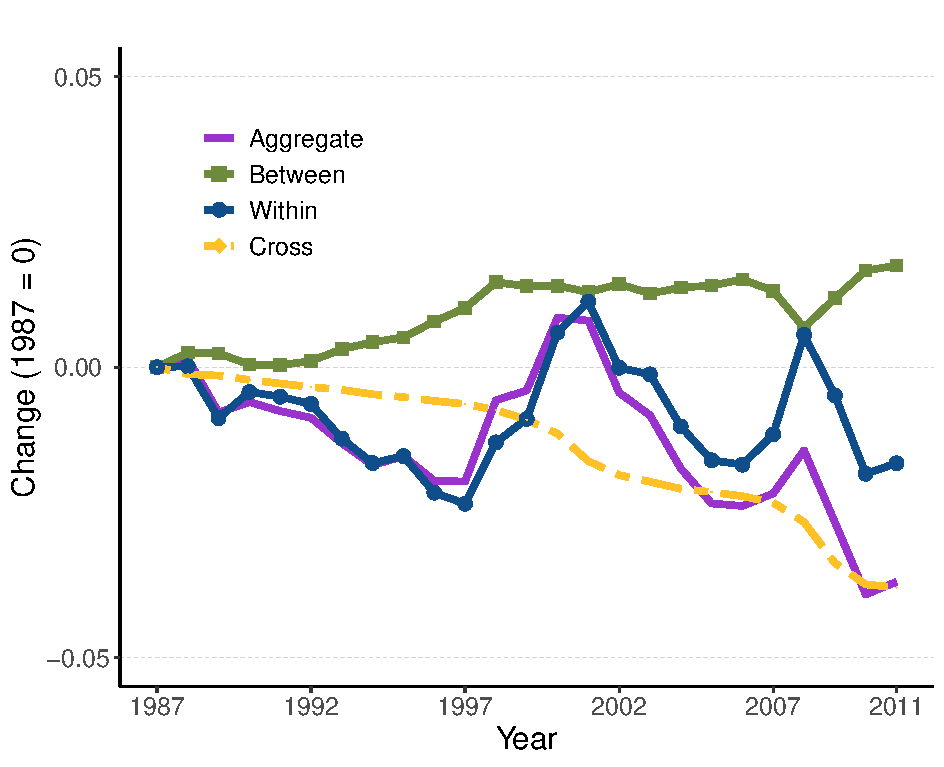
\includegraphics[width=.45\linewidth]{Appendix/Figures/elsby_hw_D_graph.pdf}}
\subfloat[NAICS 2-digit sectors]{\label{fig:elsby_hw}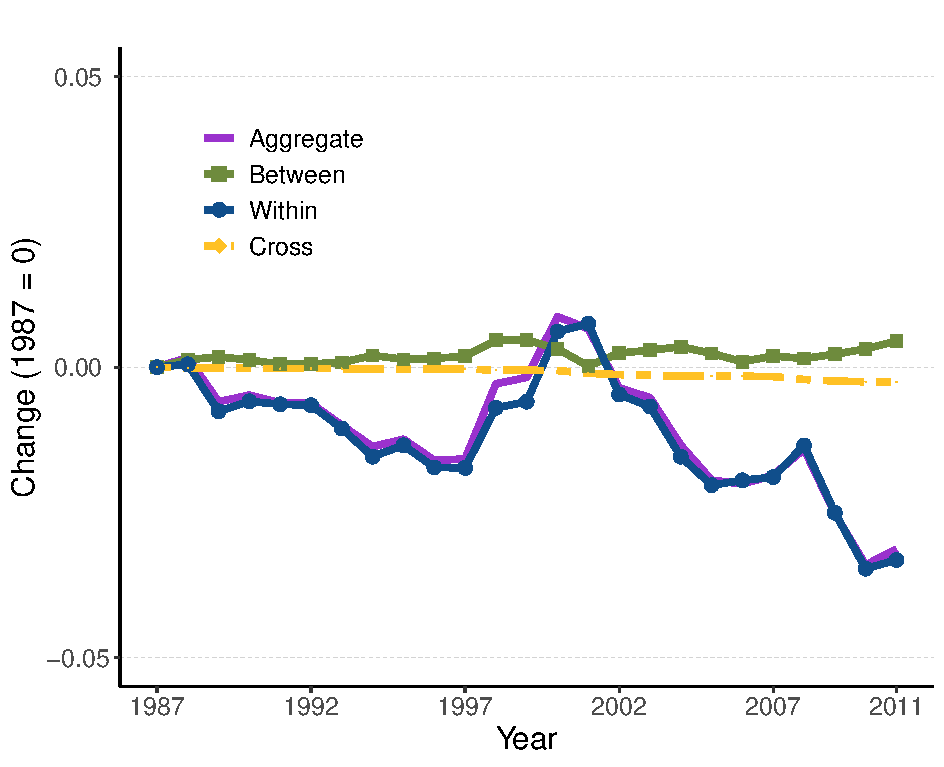
\includegraphics[width=.45\linewidth]{Appendix/Figures/elsby_hw_D_MINOR_MAJOR_graph.pdf}}\vfill
\begin{minipage}{\linewidth}
\captionsetup{justification=raggedright,singlelinecheck=false}
    \caption*{\textit{Notes}: Cumulative between, within, cross terms for the Haltiwanger method using the payroll labour share. The left panel uses data at the NAICS 3-digit level (60 sectors) and the right panel uses the same data but aggregated into NAICS 2-digit level (10 sectors). `0.05' on the y-axis corresponds to 5 percentage points (pp). \\
    \textit{Source}: BEA and the \citet{elsbyDeclineLaborShare2013a} replication package.}
\end{minipage}
\label{fig:minormajor}
\end{figure}

\subsection{What Is The Cumulative Haltiwanger Cross Contribution For Each Sector? \label{sec: veil}}

For each sector, I sum the cross contribution over each year of the `payroll labour share' sample
\begin{equation*}
    \underbrace{\sum_{t=1}^{T}\Delta\omega_{jt}\Delta\lambda_{jt}}_\text{Haltiwanger: Cross} 
\end{equation*}
Figure \ref{fig:veil} shows the cumulative Haltiwanger cross contribution is negative for virtually every sector. The reason is that, holding labour income $WL_{it}^{p}$ constant, changes in value-added $VA_{it}$ generate opposite movements in a sector's weight and labour share: $\Delta\omega_{it} > 0 \implies \Delta\lambda_{it} < 0$.

\begin{figure}[h]
  \centering
  \caption{\normalsize Size of cumulative cross contribution for each sector}
  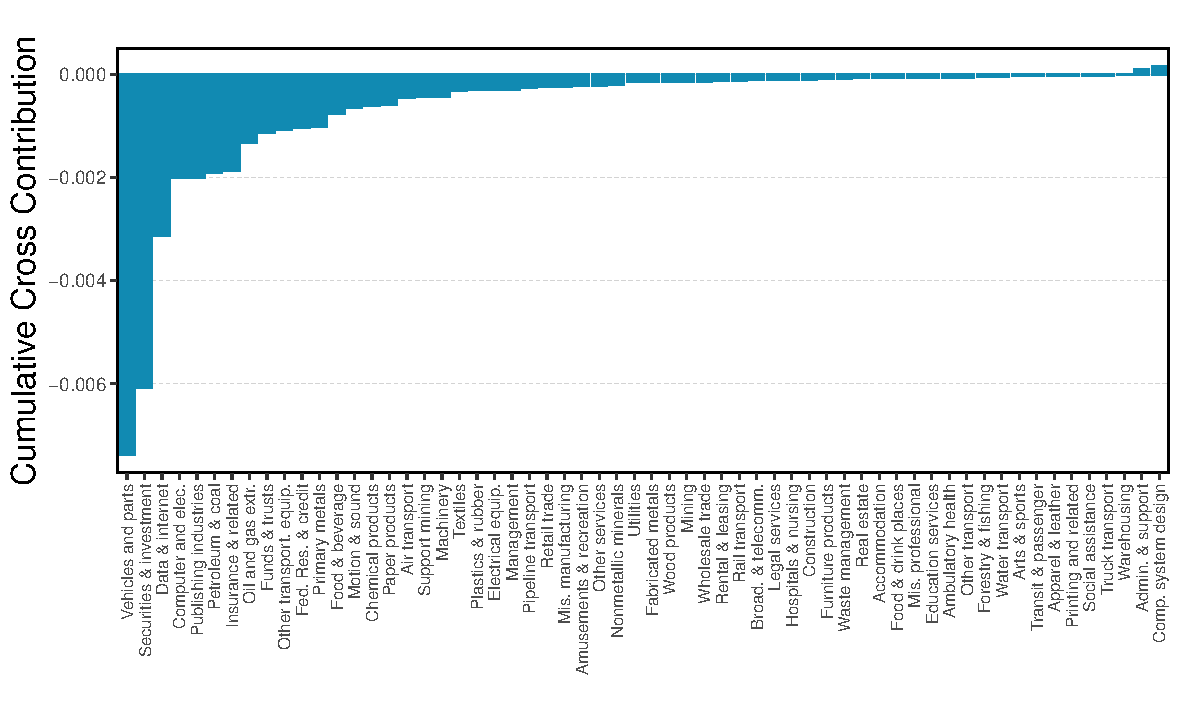
\includegraphics[width=14cm]{Decomposition/elsby_veil_total.pdf}
\begin{minipage}{\linewidth}
\captionsetup{justification=raggedright,singlelinecheck=false}
    \caption*{\textit{Notes}: Each bar indicates the cumulative sum of each sector's Haltiwanger cross contribution
  \begin{equation*}
    \underbrace{\sum_{t=1}^{T}\Delta\omega_{jt}\Delta\lambda_{jt}}_\text{Haltiwanger: Cross} 
  \end{equation*} \\
    \textit{Source}: BEA, \citet{elsbyDeclineLaborShare2013a} replication package, and author's calculations.}
\end{minipage}
  \label{fig:veil}
\end{figure}

\newpage 
\section{Theorem \ref{theorem_1} Proof \label{sec:appendix:first}}
\renewcommand{\thetable}{B\arabic{table}}
\setcounter{table}{0}
\renewcommand{\thefigure}{B\arabic{figure}}
\setcounter{figure}{0}

% \subsection{Theorem \ref{theorem_1} Proof \label{sec: theorem_1_proof}}

\noindent The Haltiwanger decomposition for the change in the labour share, $\Delta \lambda_{t} = \lambda_{t} - \lambda_{t-1}$, is
\begin{equation*}
    \Delta \lambda_{t} = \underbrace{\sum_{i=1}^{N}\Delta\omega_{it}\lambda_{it-1}}_\text{Between} + \underbrace{\sum_{i=1}^{N}\omega_{it-1}\Delta\lambda_{it}}_\text{Within} + \underbrace{\sum_{i=1}^{N}\Delta\omega_{it}\Delta\lambda_{it}}_\text{Cross}
\end{equation*}
in which $\Delta x_{it} = x_{it} - x_{it-1}$. Divide the `Cross' term into two
\begin{equation}
    \Delta \lambda_{t} = \underbrace{\sum_{i=1}^{N}\Delta\omega_{it}\lambda_{it-1}}_\text{Between} + \underbrace{\sum_{i=1}^{N}\omega_{it-1}\Delta\lambda_{it}}_\text{Within} + \underbrace{\frac{1}{2}\sum_{i=1}^{N}\Delta\omega_{it}\Delta\lambda_{it}}_\text{$\equiv$ Cross: A} + \underbrace{\frac{1}{2}\sum_{i=1}^{N}\Delta\omega_{it}\Delta\lambda_{it}}_\text{$\equiv$ Cross: B}.
\label{eqn:haltiwanger_split}
\end{equation}
Add `Cross: A' to the `Within' component in equation (\ref{eqn:haltiwanger_split})
\begin{equation*}
\begin{split}
    &= \frac{1}{2}\sum_{i=1}^{N}\Delta\omega_{it}\Delta\lambda_{it} + \sum_{i=1}^{N}\omega_{it-1}\Delta\lambda_{it} \\
    &= \sum_{i=1}^{N}\frac{\Delta\omega_{it}}{2}\Delta\lambda_{it} + \sum_{i=1}^{N}\omega_{it-1}\Delta\lambda_{it}. \\
\end{split}
\end{equation*}
Collect like terms
\begin{equation}
\begin{split}
    &= \sum_{i=1}^{N}\bigg(\frac{\Delta\omega_{it}}{2} + \omega_{it-1}\bigg)\Delta\lambda_{it} \\
    &= \sum_{i=1}^{N}\bigg(\frac{\omega_{it} - \omega_{it-1}}{2} + \omega_{it-1}\bigg)\Delta\lambda_{it} \\
    &= \sum_{i=1}^{N}\bigg(\frac{\omega_{it} + \omega_{it-1}}{2}\bigg)\Delta\lambda_{it} \\
    &= \sum_{i=1}^{N}\tilde{\omega}_{it}\Delta\lambda_{it} \\
\end{split}
\label{eqn:Shift_derivation}
\end{equation}
in which I denote $\tilde{x}_{it}$ as the arithmetic mean of $x_{it-1}$ and $x_{it}$. The last line in equation (\ref{eqn:Shift_derivation}) is the within-sector term in shift-share decomposition. Next, add `Cross: B' to the `Between' component in equation (\ref{eqn:haltiwanger_split})
\begin{equation*}
\begin{split}
    &= \frac{1}{2}\sum_{i=1}^{N}\Delta\omega_{it}\Delta\lambda_{it} + \sum_{i=1}^{N}\Delta\omega_{it}\lambda_{it-1} \\
    &= \sum_{i=1}^{N}\Delta\omega_{it}\frac{\Delta\lambda_{it}}{2} + \sum_{i=1}^{N}\Delta\omega_{it}\lambda_{it-1}. \\
\end{split}
\end{equation*}
Collect like terms
\begin{equation}
\begin{split}
    &= \sum_{i=1}^{N}\bigg(\frac{\Delta\lambda_{it}}{2} + \lambda_{it-1}\bigg)\Delta\omega_{it} \\
    &= \sum_{i=1}^{N}\bigg(\frac{\lambda_{it} - \lambda_{it-1}}{2} + \lambda_{it-1}\bigg)\Delta\omega_{it} \\
    &= \sum_{i=1}^{N}\bigg(\frac{\lambda_{it} + \lambda_{it-1}}{2}\bigg)\Delta\omega_{it} \\
    &= \sum_{i=1}^{N}\Delta\omega_{it}\tilde{\lambda}_{it} \\
\end{split}
\label{eqn:Share_derivation}
\end{equation}
in which $\tilde{x}_{it}$ denotes the arithmetic mean of $x_{it-1}$ and $x_{it}$. The last line in equation (\ref{eqn:Share_derivation}) is the between-sector term in the shift-share decomposition. \qed


% \subsection{Reallocation Effect With Payroll Labour Share \label{sec: reallocation_payroll}}

The reallocation effect is zero when using the shift-share decomposition instead of the Haltiwanger decomposition in the `payroll labour share' definition (see Table \ref{tab:rr}). By Theorem \ref{theorem_1}, the shift-share between-effect is small (downward biased) when the cross-term is large and negative. For the shift-share between term to be `more' undercounted than in samples that include self-employed income, we require
\begin{equation*}
    \sum_{i=1}^{N} \Delta\omega_{i}\Delta\lambda_{i}^{p} < \sum_{i=1}^{N} \Delta\omega_{i}\Delta\lambda_{i}
\end{equation*}
in which both terms are less than zero, as in the data. The total labour share $\lambda_{i}$ satisfies
\begin{equation}
    \lambda_{i} = \lambda_{i}^{p} + \lambda_{i}^{s}
\label{eqn:labour_share_definition}
\end{equation}
where $\lambda_{i}^{p}$ and $\lambda_{i}^{s}$ are the payroll and self-employed labour shares in sector $i$, respectively. 

To simplify, suppose $N = 2$ and that sector 1 is growing as a share of value-added. Then
\begin{equation}
\begin{split}
    \Delta\omega_{1}\Delta\lambda_{1}^{p} + \Delta\omega_{2}\Delta\lambda_{2}^{p} &< \Delta\omega_{1}\Delta\lambda_{1} + \Delta\omega_{2}\Delta\lambda_{2} \\ 
    \Delta\omega_{1}\Big(\Delta\lambda_{1}^{p} - \Delta\lambda_{i}\Big) &< \Delta\omega_{2}\Big(\Delta\lambda_{2} -\Delta\lambda_{2}^{p}\Big) \\ 
    \Delta\omega_{1}\Big(\Delta\lambda_{1}^{p} - \Delta\lambda_{i}\Big) &< \Delta\omega_{1}\Big(\Delta\lambda_{2}^{p} -\Delta\lambda_{2}\Big) \\ 
    \Delta\lambda_{1}^{p} - \Delta\lambda_{i} &< \Delta\lambda_{2}^{p} -\Delta\lambda_{2} \\ 
\end{split}
\end{equation}
Using definition (\ref{eqn:labour_share_definition})
\begin{equation}
\begin{split}
    \Delta\lambda_{1}^{p} - \Delta\lambda_{i} &< \Delta\lambda_{2}^{p} -\Delta\lambda_{2} \\ 
    -\Delta\lambda_{1}^{s} &< -\Delta\lambda_{2}^{s} \\ 
    \Delta\lambda_{1}^{s} &> \Delta\lambda_{2}^{s}
\end{split}
\label{eqn:self_emp_condition}
\end{equation}
So, the outlier present in table \ref{tab:rr} arises when the change in the self-employed labour share is larger (more negative) in the shrinking sector. Translated into the sixty-sector-setting, (\ref{eqn:self_emp_condition}) implies the self-employed labour share should fall more in shrinking sectors in, for example, the Manufacturing and Trade, Transportation and Utilities supersectors. Intuitively, if (\ref{eqn:self_emp_condition}) holds then the size of the cross-term becomes more positive because the total labour share falls by more than the payroll labour share in shrinking sectors. 


% \newpage
% \section{Appendix Two
% \label{sec:appendix:two}}
% \renewcommand{\thetable}{C\arabic{table}}
% \setcounter{table}{0}
% \renewcommand{\thefigure}{C\arabic{figure}}
% \setcounter{figure}{0}

\printbibliography

\end{document}
